\chapter{Antecedentes}

\section{Marco Teórico}

\subsection{Ecosistema PropTech}

El ecosistema PropTech (acrónimo de Property Technology) representa una pieza fundamental dentro de la transformación digital de la industria inmobiliaria. Este fenómeno describe un movimiento que está impulsando un cambio de mentalidad profundo tanto dentro de la industria de bienes raíces como en sus consumidores. Dicho cambio se centra en la innovación impulsada por la tecnología para la recopilación de datos, las transacciones y el diseño de edificios y ciudades (Baum y Dearsley, 2021, citado en Tagliaro et al., 2024). El PropTech se define como la implementación masiva de tecnologías emergentes dentro del sector inmobiliario. Abarca un espectro muy amplio de aplicaciones, incluyendo herramientas de emparejamiento de viviendas, drones, realidad virtual, modelado de información de construcción (BIM), análisis de datos, inteligencia artificial (IA), Internet de las Cosas (IoT), contratos inteligentes, blockchain, crowdfunding sectorial, ciudades inteligentes, hogares inteligentes y economía colaborativa \parencite{SiniakEtAl2020}. Su impacto en el mercado es innegable: en la última década, el sector PropTech ha experimentado un aumento superior al 300\% y, en la actualidad, cuenta con más de 8.000 empresas a nivel mundial que proporcionan soluciones enfocadas en la tecnología (JLL, 2021, citado en Tagliaro et al., 2024). De acuerdo con los sistemas de clasificación sectorial (como NACE rev.2), el PropTech es un fenómeno complejo que va más allá de la simple convergencia entre el sector inmobiliario y el tecnológico. Su núcleo de actividad suele concentrarse fuertemente en el sector de ``Información y comunicación'', abarcando el desarrollo de portales web y actividades de programación informática (Tiwari y Shukla, 2022, citado en Tagliaro et al., 2024).). Por lo tanto, el término sirve como un concepto colectivo para determinar a aquellas start-ups y plataformas que ofrecen productos tecnológicamente innovadores y nuevos modelos de negocio para los mercados inmobiliarios, incidiendo en todas las etapas del ciclo de vida de un activo, desde su construcción hasta su venta, alquiler o gestión (Nikolai Siniak et al., 2020; Braesemann y Baum, 2020).

\subsubsection{Evolución histórica y categorización tecnológica}

El análisis de la innovación en bienes raíces se ha centrado predominantemente en el desarrollo tecnológico bajo el supuesto de que este mejora los procesos comerciales y de construcción (Baum, 2017; Baum et al., 2020, citados en Tagliaro et al., 2024). Según estos autores, la innovación impulsada por la tecnología en el sector inmobiliario se ha producido a través de tres olas sucesivas:

\begin{itemize}
\item \textbf{PropTech 1.0:} Introdujo los datos y la potencia informática elemental en el sector, ejemplificado por herramientas pioneras como el software AutoCAD.
\item \textbf{PropTech 2.0:} Se enfocó en alinear la demanda del mercado con la oferta inmobiliaria, apoyándose fuertemente en el comercio electrónico y en los enfoques basados en redes sociales.
\item \textbf{PropTech 3.0:} Representa la etapa actual, impulsada por las presiones globales del cambio climático, la rápida urbanización y los cambios demográficos. Esta ola está liderada por la integración de tecnologías exógenas como el Internet de las Cosas (IoT), el Aprendizaje Automático (ML), la Inteligencia Artificial (IA) y Blockchain (Baum, 2017; Davenport, 2019 citado en Baum et al., 2020).
\end{itemize}

Para comprender la estructura de este mercado tecnológico, la literatura propone diversas categorizaciones. Por ejemplo, Braesemann y Baum (2020) proponen agrupar la tecnología PropTech en seis clústeres principales que concentran las 30 tecnologías más relevantes:

\begin{itemize}
\item Smart Real Estate (inmuebles inteligentes, basados principalmente en tecnología de sensores).
\item Data Analytics (analítica de datos, incluyendo valoración automatizada, mapeo, Big Data e IA).
\item Modelling (modelado, incluyendo representaciones digitales de edificios como BIM y VR/AR).
\item Real Estate Fintech (tecnología financiera aplicada, como crowdfunding, blockchain y criptomonedas).
\item Business Processes (gestión de procesos de negocio, flujos de trabajo, CRM y chatbots).
\item ConTech (tecnología de construcción, incluyendo prefabricación y construcción modular).
\end{itemize}

\begin{figure}[htbp]
\centering
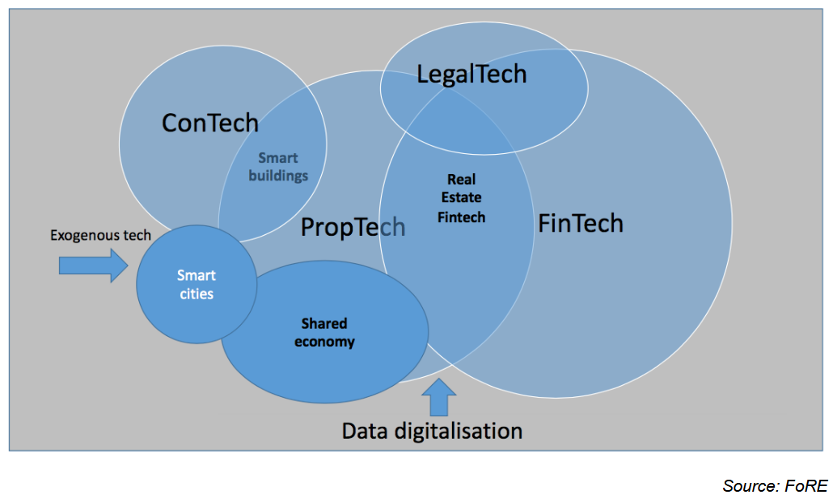
\includegraphics[width=0.90\textwidth]{figures/word/image8.png}
\caption{Esquema PropTech 2020.}
\end{figure}

Fuente: \parencite{BaumEtAl2020}

\subsubsection{La economía de los datos y el cambio de valor}

Quizás el impacto más disruptivo del ecosistema PropTech radica en cómo ha transformado la percepción de valor dentro del sector. Tradicionalmente centradas en los activos físicos (el ``ladrillo y mortero''), las transacciones y evaluaciones inmobiliarias están experimentando una transferencia de valor hacia los activos intangibles, específicamente, hacia los datos (Landau-Ward y Porter, 2019 citados en Braesemann y Baum, 2020). El PropTech incrementa drásticamente la información disponible sobre los edificios y el entorno construido a través del fenómeno de la datificación (Meyer-Schonberger y Cukier, 2012, citados en Tagliaro et al., 2024; Braesemann y Baum, 2020). En este contexto digitalizado, los datos ya no son un subproducto del proceso inmobiliario, sino que se convierten en una mercancía comercializable (tradeable commodity) y en el recurso central del mercado \parencite{BraesemannBaum2020}. Tecnologías específicas como la nube (cloud computing), la Inteligencia Artificial y las Interfaces de Programación de Aplicaciones (API) de acceso abierto permiten agregar información del sector en tiempo real y a gran escala, habilitando el acceso al Big Data inmobiliario ---datos producidos a alta velocidad, variedad y volumen--- que los modelos de hojas de cálculo tradicionales no pueden procesar (Davenport, 2019, citado en Baum et al., 2020). Esta acumulación y procesamiento de datos resulta fundamental porque la información procesada es esencialmente el servicio que añade valor para los usuarios contemporáneos \parencite{BraesemannBaum2020}. Esto se evidencia en la proliferación de Modelos de Valoración Automatizada (AVM), los cuales utilizan Machine Learning y Big Data para predecir precios basándose en información pública, espacial y económica, mejorando la transparencia, la liquidez y reduciendo los tiempos de transacción en el mercado (Davenport, 2019, citado en Baum et al., 2020).

\subsubsection{Resistencia al cambio y el enfoque ``Human-Tech''}

A pesar de la irrupción tecnológica, el sector inmobiliario es históricamente lento para adoptar la innovación, favoreciendo las innovaciones incrementales por sobre los cambios radicales (Tiwari y Shukla, 2022, citado en Tagliaro et al., 2024). Esta resistencia suele fundamentarse en actitudes conservadoras y en dinámicas especulativas de redes cerradas donde aún se extraen altos rendimientos sin necesidad de innovar \parencite{SiniakEtAl2020}. Actualmente, las empresas que se basan en sistemas digitalizados a menudo lo hacen utilizando software genérico, con altos porcentajes de ejecutivos admitiendo que sus firmas continúan usando hojas de cálculo convencionales como su herramienta principal para valuaciones, análisis de flujo de caja y pronósticos (Altus, 2019; RICS, 2019, citados en Baum et al., 2020). Sin embargo, el sector enfrenta una presión creciente para adaptarse. El desafío principal radica en equilibrar la contribución de las nuevas tecnologías con el enfoque tradicional de resolución de problemas, logrando que la transición digital no interrumpa excesivamente las operaciones actuales (Tiwari y Shukla, 2022, citado en Tagliaro et al., 2024). Para lograrlo, la industria está convergiendo hacia un modelo human-tech (humano-tecnológico). En este modelo, la tecnología no se percibe como un sustituto del valor humano, sino como una herramienta que hace que la información sea más accesible y transparente (Tiwari y Shukla, 2022, citado en Tagliaro et al., 2024, que incluyen datos de la entrevista INT-10). En este escenario, la tecnología es interpretada simplemente como ``un tenedor'' (like a fork): una herramienta útil para facilitar la innovación, pero que debe ser dirigida y conducida por humanos. Al delegar las tareas repetitivas y automatizables (como la lectura y extracción masiva de datos) a las máquinas, los profesionales pueden reducir errores, disminuir costos y reenfocar su tiempo hacia actividades de mayor valor agregado, como la toma de decisiones basada en evidencia, la evaluación de nuevos modelos de negocio y la consultoría estratégica para clientes e inversores (Moss, 2018, citado en Baum et al., 2020; Tiwari y Shukla, 2022, citado en Tagliaro et al., 2024).

\subsection{Asimetría de la Información en el Real Estate}

Históricamente, el mercado inmobiliario se ha caracterizado por operar bajo condiciones de alta incertidumbre y baja visibilidad. Las transacciones de bienes raíces ocurren habitualmente dentro de sistemas de información altamente opacos, a menudo sin que la información relevante sea distribuida de forma pública a través de fuentes oficiales (Juneja, 2019). Esta falta de claridad no solo hace que los procesos actuales sean ineficientes, sino que genera una profunda asimetría de información que permite a ciertos actores del mercado participar en el uso de información privilegiada (insider trading), lo que conduce inevitablemente a un falso equilibrio del mercado (Kurlat y Stroebel, 2015, citado en Baum et al., 2020). Este fenómeno encuentra su raíz teórica en el concepto del mercado de los ``limones'' desarrollado por George Akerlof en 1970, quien ganó el premio Nobel de Economía en el año 2001. Según este autor, en un mercado caracterizado por la incertidumbre sobre la calidad y la asimetría de información, los vendedores poseen un mayor conocimiento sobre el estado real del bien que los compradores. Dado que al comprador le resulta imposible distinguir con certeza entre un producto de buena calidad y uno defectuoso (denominado ``limón''), ambos tienden a venderse al mismo precio. Esto genera un incentivo para comercializar bienes de calidad inferior, lo que provoca una reducción en la calidad promedio y en el tamaño del mercado. En definitiva, los productos defectuosos tienden a expulsar a los buenos, y el costo de esta dinámica radica en que los negocios legítimos terminan siendo desplazados \parencite{Akerlof1970}. Al trasladar este modelo teórico al mercado inmobiliario, el ``limón'' se traduce en propiedades con vicios ocultos o precios inflados. En este sector, la asimetría se manifiesta de forma estructural: el vendedor o propietario conoce el historial real del inmueble (problemas de humedad, conflictos consorciales, etc.) y el comportamiento reciente de su zona. Por el contrario, el comprador o inquilino, salvo que cuente con asesoramiento profesional, opera con información parcial y desactualizada. Dado que al usuario le resulta extremadamente difícil distinguir a simple vista si el precio solicitado es justo o si la propiedad es de ``buena calidad'' sin vivir en ella, se genera el mismo falso equilibrio del que hablaba Akerlof. A nivel operativo, la incertidumbre sobre el valor real de una propiedad retrasa significativamente el proceso inicial de venta. Esta falta de certezas aumenta el riesgo de sufrir prácticas desleales en las negociaciones (como el gazumping, donde el vendedor acepta a último momento una oferta superior tras haber acordado una venta) y prolonga excesivamente el tiempo destinado a cerrar un acuerdo.

\subsubsection{Transparencia como motor de eficiencia}

La transferencia eficiente de la propiedad requiere altos niveles de transparencia para que los participantes del mercado puedan acceder a los datos necesarios y así tomar decisiones racionales (Schulte et al., 2005, citado en Baum et al., 2020). Sin una transparencia elevada, los mercados inmobiliarios simplemente no pueden funcionar de manera eficiente \parencite{SiniakEtAl2020}. Al mejorar la visibilidad de la información, se minimizan los factores adversos vinculados a la iliquidez de los activos y se aceleran las velocidades de transacción. Para medir y comparar este fenómeno a nivel mundial, se utiliza el Índice Global de Transparencia Inmobiliaria (Global Real Estate Transparency Index o GRETI). Según la literatura, las economías emergentes suelen carecer de la transparencia necesaria para optimizar sus mercados \parencite{SiniakEtAl2020}. De acuerdo con la última edición del reporte bianual GRETI en el año 2024, Argentina se posiciona en el puesto 52 a nivel global con una puntuación de 3.36, lo que clasifica a la economía del país como un mercado ``semi-transparente'' \parencite{JLL2024}. Al desglosar este indicador, se observa un desempeño dispar que justifica las ineficiencias del sector a nivel local. Si bien el país presenta una posición relativa mejor en el rubro de vehículos listados (puesto 46) y en su marco legal y regulatorio (puesto 48), exhibe un retraso crítico en áreas operativas fundamentales: ocupa el puesto 53 en fundamentos de mercado, el 55 en sostenibilidad, el 62 en el desempeño de las inversiones, y cae drásticamente hasta el puesto 66 en lo que respecta al proceso de transacciones \parencite{JLL2024}. Esta falta de transparencia plena y el déficit en el procesamiento de transacciones resultan críticos, ya que incorporar objetivos de desempeño digital, información objetiva de inversión y crecimiento sostenible en las prácticas operativas es un requisito fundamental, entendiendo que los mercados de tierras y edificios son tanto una precondición como una consecuencia del crecimiento económico.

\subsubsection{Sesgos de datos y nuevas desigualdades digitales}

A medida que el mercado inmobiliario y de alquileres se traslada al entorno en línea, surge una nueva problemática. Si bien internet ayuda a democratizar el acceso a la información, no necesariamente iguala su suministro. La autoselección tecnológica y los sesgos en la oferta de información construyen nuevas desigualdades digitales que dan forma a los costos de búsqueda de vivienda, a los conjuntos de opciones disponibles y a los patrones de clasificación residencial. Estos sesgos no solo impactan en la equidad de la información para los usuarios finales, sino que también alteran las conclusiones que los investigadores de vivienda y los formuladores de políticas públicas pueden extraer del mundo real a partir de datos colaborativos o crowdsourced data (Arribas-Bel y Bakens, 2018; Folch et al., 2018; McLaughlin y Young, 2018; Narayanan y MacDonald, 2019, citado en Boeing, 2019). Hoy en día, las plataformas tecnológicas forjan instituciones emergentes con una inmensa capacidad para remodelar las economías urbanas y los paisajes de información, pudiendo agravar estas asimetrías si no se gestionan correctamente.

\subsubsection{El rol nivelador del PropTech}

Frente a estas barreras de información, el ecosistema PropTech se posiciona como el principal agente para hacer que el mercado de bienes raíces sea más seguro y transparente (citado en Tagliaro et al., 2024, que incluyen datos de la entrevista INT-10). La creciente accesibilidad a las nuevas tecnologías permite superar la ``fricción del espacio'' que, de otro modo, conduciría a condiciones de arbitraje espacial y ventajas injustas para quienes poseen la información \parencite{SiniakEtAl2020}. La tecnología permite imaginar un escenario ideal en el cual los posibles compradores de viviendas puedan acudir a una única plataforma donde se enumeren todas las propiedades del mercado, acompañadas de una valoración independiente y pública, la cual sea descubrible tanto para el vendedor como para el comprador y los prestamistas. Al democratizar el acceso a los datos, el PropTech tiene el potencial de nivelar el campo de juego, acelerando el proceso de transacción y mejorando radicalmente la liquidez de esta enorme clase de activos a nivel mundial.

\subsection{Teoría de los Precios Hedónicos}

El mercado inmobiliario presenta el desafío intrínseco de que cada propiedad es única y heterogénea. Para abordar la valoración técnica de estos bienes complejos, el enfoque metodológico más aceptado y ampliamente utilizado en la investigación durante décadas es la función de precios hedónicos, descrita originalmente por Sherwin Rosen en 1974. Esta teoría constituye la base de los modelos de valoración modernos y se apoya en la premisa de que los bienes son típicamente vendidos como un paquete de atributos inherentes. En consecuencia, el precio total de una propiedad puede explicarse y predecirse calculando la suma de los precios implícitos de las características individuales asociadas a la misma \parencite{Rosen1974}. Bajo este marco, los modelos de precios hedónicos no comienzan evaluando la propiedad de forma aislada, sino que parten del análisis de la información existente sobre cualquier propiedad disponible en el mercado. De esta manera, el valor de la vivienda se modela customarily mediante modelos de regresión hedónica, en los cuales el precio es explicado por una combinación de atributos estructurales (tales como el tamaño, cantidad de habitaciones o año de construcción) y atributos de localización (ubicación geográfica y características del entorno). Esta desagregación permite a los analistas extraer conclusiones matemáticas sobre cómo la variación de un atributo individual impacta en el valor final del inmueble.

\subsubsection{Implementación en Modelos de Valoración Automatizada (AVM)}

La adopción práctica de la teoría hedónica ha dado lugar a los Modelos de Valoración Automatizada (AVM). Para funcionar, los AVM hedónicos requieren información detallada sobre los atributos básicos de la propiedad, la extensión de las mejoras de capital y las características locacionales. Estos modelos típicamente incorporan un motor de búsqueda que compara los atributos de la propiedad objetivo con propiedades comparables, utilizando un patrón de búsqueda radial u otros parámetros lógicos dentro de un período de tiempo predeterminado (Eichholtz, Kok y Quigley, 2010, citado en Kok et al, 2017). Desde un punto de vista matemático, la estimación del valor en estos modelos se fundamenta en la Regresión Lineal Múltiple, cuya especificación formal para la valoración de activos inmobiliarios es:

\[
Y_i = \beta_0 + \beta_1 x_{i1} + \cdots + \beta_k x_{ik} + u_i
\]

En esta expresión, Y representa la variable dependiente, es decir, el valor o precio estimado de la propiedad. Por su parte, $\beta$0 actúa como la constante o intersección del modelo, mientras que los coeficientes $\beta$i definen los ``precios implícitos'' o el peso relativo de cada característica (como metros cuadrados, ubicación o estado del inmueble). Estas características son capturadas por las variables independientes Xi, que engloban los atributos estructurales y locacionales. Finalmente, el término $\epsilon$ contabiliza el error estadístico inherente a la variabilidad no observada por el modelo \parencite{AbidoyeChan2018}. Los AVM basados en modelos hedónicos son extremadamente comunes en la actualidad debido a que se apoyan en modelos de regresión simples, los cuales resultan fáciles de implementar a nivel informático y sencillos de comprender para los actores del mercado que no poseen un perfil técnico, facilitando así la adopción de estas tecnologías.

\subsubsection{Limitaciones del enfoque clásico y la adopción de Machine Learning}

A pesar de su extensa aplicabilidad, el modelo hedónico tradicional presenta limitaciones operativas frente a la complejidad de los mercados urbanos. Su principal desventaja es que los modelos de regresión clásicos son modelos globales. Esto significa que generan una única fórmula predictiva que permanece constante a lo largo de todo el rango de variables, asumiendo un comportamiento uniforme para los atributos de la propiedad, las comodidades y los datos contextuales. Sin embargo, la realidad de los bienes raíces demuestra que muchas variables tienen una relación no lineal con respecto al valor predicho. Por lo tanto, un único modelo matemático global rara vez tiene éxito al predecir el valor de la propiedad con el grado de precisión óptimo exigido por el mercado actual. Para superar estas limitaciones, los sistemas modernos de valoración han evolucionado hacia el uso del Aprendizaje Automático (Machine Learning). Específicamente, destacan los modelos de árboles de decisión (decision tree models). En lugar de aplicar una única fórmula general, estos modelos dividen el conjunto de datos masivos (dataset) en subconjuntos más pequeños y granulares, aplicando un modelo de regresión independiente a cada uno de ellos. El punto de división dentro del nodo raíz se determina mediante la aplicación de una función de costo que minimiza la varianza en una línea de regresión para ambos subconjuntos. Esta capacidad de segmentación permite al algoritmo capturar la naturaleza no lineal y dinámica de los precios inmobiliarios de una manera mucho más exacta que la valuación humana o estadística convencional. A diferencia de la regresión lineal tradicional, los modelos de árboles de decisión (y sus variantes ensemble como XGBoost) aprenden mediante la partición recursiva del espacio de características. En cada nodo, el algoritmo selecciona la división que minimiza la suma de los errores cuadrados, utilizando como función de costo el Error Cuadrático Medio (MSE). Esta métrica cuantifica la diferencia entre el valor real de la propiedad (Yi) y la predicción del modelo (Y\textasciicircum{}i), penalizando severamente las desviaciones grandes:

\[
\operatorname{MSE}=\frac{1}{n}\sum_{i=1}^{n}\left(Y_i-\hat{Y}_i\right)^2
\]

Al minimizar esta función de costo, el modelo ajusta sus parámetros para lograr una mayor precisión predictiva, adaptándose a las no linealidades complejas del mercado inmobiliario que los modelos estadísticos simples no logran capturar \parencite{KokEtAl2017}.

\subsection{Sistemas de Valuación Automatizada (AVM)}

Un Sistema de Valuación Automatizada (AVM, por sus siglas en inglés) es un servicio tecnológico que utiliza modelos matemáticos para proporcionar el valor estimado de una propiedad en un momento específico en el tiempo \parencite{ElJaouhariEtAl2024}. Estos sistemas asumen una relación constante entre el valor del inmueble y diversas variables independientes dentro de un mercado determinado. Tradicionalmente, estos modelos asumían una relación constante entre el valor y las variables independientes del mercado; sin embargo, en su estado del arte actual, los AVM integran algoritmos de Aprendizaje Automático (Machine Learning) para realizar predicciones sobre el precio basándose en datos espaciales, económicos e inmobiliarios \parencite{FaxvaagEtAl2025}. Al capitalizar el uso de macrodatos (Big Data), estos modelos permiten una valoración dinámica y escalable que procesa información en tiempo real. Esta capacidad es fundamental para mitigar el stale valuation problem (problema de valuación obsoleta) que caracteriza a los enfoques tradicionales, donde la tasación humana se ve limitada por la frecuencia de actualización de los datos (Faxvaag et al., 2025; El Jaouhari et al., 2024). Asimismo, Glumac y Des Rosiers (2018) sostienen que la evolución de los AVM ha trascendido el enfoque empírico inicial hacia un marco conceptual riguroso. Estos autores proponen una taxonomía que clasifica a los AVM no solo por su capacidad predictiva, sino por su rol como sistemas de apoyo a la decisión (Decision Support Systems). Este enfoque respalda la arquitectura de Nidio, la cual integra datos estructurados con análisis geoespaciales para reducir la subjetividad inherente a las valuaciones convencionales, transformando la tasación en un proceso fundamentado y transparente.

\subsubsection{Evolución algorítmica: De la regresión a los árboles de decisión}

Si bien los modelos hedónicos clásicos se basan en regresiones simples, la necesidad de mayor precisión ha llevado al desarrollo de algoritmos basados en el aprendizaje automático (Birkeland et al., 2021, citado en Faxvaag et al., 2025). Entre las técnicas predictivas más destacadas se encuentran los modelos de árboles de decisión. Estos árboles presentan múltiples ventajas operativas: son computacionalmente eficientes, facilitan el cálculo de la significancia estadística y poseen la capacidad intrínseca de manejar variables categóricas sin necesidad de transformaciones manuales complejas \parencite{Babtan2024}. Sin embargo, la literatura advierte que los árboles de decisión individuales son propensos al sobreajuste (overfitting). Si crecen sin restricciones, memorizan el ``ruido'' de los datos de entrenamiento y pierden su capacidad de generalización frente a datos nuevos, resultando en predicciones deficientes \parencite{BirkelandEtAl2021}.

\subsubsection{Modelos de ensamble: Random Forest y XGBoost}

Para superar las limitaciones de los árboles individuales, los AVM modernos utilizan técnicas de ensamble (ensemble methods), las cuales combinan múltiples árboles para generar una única predicción robusta \parencite{BirkelandEtAl2021}. Dentro de estas metodologías avanzadas, destacan dos enfoques en el ecosistema PropTech: Random Forest: Desarrolla múltiples árboles de decisión independientes seleccionando variables aleatorias y utilizando muestras bootstrapped. La predicción final resulta de promediar los resultados de toda la colección de árboles, lo cual es altamente efectivo para reducir la varianza y mitigar el sobreajuste \parencite{BirkelandEtAl2021}. Gradient Boosting y eXtreme Gradient Boosting (XGBoost): A diferencia del bosque aleatorio, los modelos de impulso por gradiente (gradient boosting) construyen árboles secuencialmente. Cada nuevo árbol se ajusta para corregir el error residual del árbol anterior. Herramientas algorítmicas extremas como XGBoost han demostrado una capacidad superior para capturar relaciones no lineales complejas en la valoración de propiedades \parencite{Babtan2024}. La literatura académica contemporánea respalda de manera contundente la adopción del método XGBoost por sobre los enfoques hedónicos clásicos. Estudios recientes que analizaron muestras masivas de propiedades han demostrado que XGBoost ofrece el mejor rendimiento predictivo general al ser comparado con técnicas tradicionales (como la Regresión Lineal OLS), logrando mejoras significativas en indicadores estadísticos clave como el Error Cuadrático Medio (RMSE) (Stang et al., 2023). Además de su precisión matemática, el entorno de XGBoost proporciona ventajas desde la ingeniería de software, dado que ofrece bibliotecas de código abierto altamente optimizadas que permiten entrenar y ajustar hiperparámetros con gran rapidez \parencite{BirkelandEtAl2021}. En contraste con otros métodos, la técnica XGBoost aplica un mecanismo que permite procesar bases de datos dispersas o datasets donde las variables tienen valores faltantes, aumentando significativamente el rendimiento del modelo frente a datos inmobiliarios reales y ruidosos \parencite{Babtan2024}. Asimismo, XGBoost ha demostrado una enorme flexibilidad técnica al permitir la integración tanto de datos estructurados tradicionales como de variables no estructuradas extraídas mediante grandes modelos de lenguaje (LLM), lo que lo posiciona como la herramienta más eficiente y escalable para la automatización masiva de valuaciones \parencite{FaxvaagEtAl2025}. A pesar de sus marcadas ventajas operativas, una limitación técnica crítica de XGBoost radica en su alta dependencia de la densidad y representatividad del conjunto de datos de entrenamiento. Al ser un algoritmo diseñado para aprender patrones complejos a partir de macrodatos (Big Data), su rendimiento predictivo óptimo se concentra en mercados urbanos densamente consolidados donde la oferta y el histórico de transacciones son abundantes. En contraposición, el modelo exhibe serias restricciones al aplicarse en entornos rurales, ciudades pequeñas o suburbios alejados; en estas regiones geográficas, la baja frecuencia de publicaciones y la escasez de datos históricos (thin markets) impiden que el algoritmo establezca parámetros lógicos de división estables, incrementando drásticamente el error de generalización y alterando los coeficientes estimados debido a sesgos por falta de muestras (Stang et al., 2023).

\subsubsection{Evaluación de rendimiento y Explicabilidad (SHAP)}

Para que un AVM sea viable en el mercado, no basta con que sea preciso; debe ser medible y explicable. El rendimiento de estos algoritmos se evalúa mediante indicadores estadísticos clave (KPIs), buscando siempre maximizar la varianza explicada y minimizar el error predictivo \parencite{ElJaouhariEtAl2024}. Por ejemplo, se utiliza la fórmula MSE mencionada anteriormente para medir el error cuadrático medio y definir la exactitud, y el coeficiente de determinación para medir la robustez del modelo:

\[
R^2 = 1 - \frac{\text{Residual sum of squares}}{\text{Total sum of squares}} = \frac{\text{SSE}}{\text{TSS}} = \frac{n\cdot \operatorname{MSE}}{\text{TSEE}}
\]

El coeficiente de determinación (R2) actúa como un indicador de bondad de ajuste, cuantificando la capacidad del modelo para capturar la variabilidad inherente a los precios del mercado inmobiliario. En la arquitectura de valuación propuesta, un valor elevado de R2 permite validar que el conjunto de variables independientes (tanto estructurales como geoespaciales) seleccionadas por el algoritmo poseen una relevancia estadística significativa para determinar el valor de los inmuebles, garantizando que el modelo trasciende una estimación basada puramente en promedios históricos \parencite{KokEtAl2017}. Finalmente, uno de los mayores desafíos técnicos de algoritmos avanzados como XGBoost es su naturaleza de ``caja negra'', lo cual choca con la necesidad de transparencia del mercado inmobiliario. Para solucionar esto y que el sistema sea interpretable, el estado del arte sugiere incorporar metodologías como SHAP (SHapley Additive exPlanations). El enfoque SHAP, fundamentado en la teoría de juegos cooperativos, permite descomponer y cuantificar exactamente cuánto contribuye cada atributo del inmueble a la predicción del precio final, devolviendo la confianza y explicabilidad al proceso de valuación \parencite{LundbergLee2017}.

\subsection{Análisis Geoespacial y Sistemas de Información Geográfica (GIS)}

El mercado inmobiliario es inherentemente espacial, ya que el valor de una propiedad está intrínsecamente ligado a su ubicación geográfica y a su entorno circundante (Stang et al., 2023). En este contexto, los Sistemas de Información Geográfica (GIS, por sus siglas en inglés) han surgido como una herramienta tecnológica fundamental para capturar, almacenar, manipular, analizar y visualizar datos con referencias espaciales. Históricamente, los modelos de valuación han utilizado atributos locacionales de manera estática. Sin embargo, la integración de herramientas GIS permite una comprensión mucho más profunda y dinámica de la distribución territorial del mercado \parencite{DrojEtAl2024}. Estos sistemas no solo facilitan la visualización de datos a través de mapas de calor o capas de zonificación, sino que habilitan el procesamiento de datos de proximidad en tiempo real, tales como la distancia a redes de transporte público, áreas verdes, centros educativos y zonas comerciales.

\subsubsection{El Análisis Multicriterio (MCDA) como soporte a la decisión}

En los problemas de localización y valuación de bienes raíces, las decisiones rara vez se basan en un único factor (como el precio por metro cuadrado). Los usuarios finales evalúan un conjunto de múltiples criterios que, a menudo, entran en conflicto entre sí. Para abordar esta complejidad matemática y espacial, la literatura académica respalda el uso del Análisis de Decisión Multicriterio basado en GIS (GIS-MCDA) \parencite{Malczewski2006}. El enfoque MCDA no consiste en calcular un promedio ponderado arbitrario, sino en establecer un marco metodológico riguroso que funciona como un sistema de soporte a la decisión \parencite{Malczewski2006}. Esta técnica permite integrar diferentes dimensiones espaciales y asignarles un ``peso'' o nivel de importancia específico. Al combinar el análisis espacial de los sistemas GIS con las matrices de decisión del MCDA, se logra transformar datos geográficos brutos en información estratégica altamente procesada y útil para el usuario.

\subsubsection{Personalización del valor mediante el entorno urbano}

La integración de las tecnologías GIS y MCDA en las plataformas PropTech modernas permite ir más allá del análisis estadístico convencional para introducir el concepto de personalización del valor inmobiliario. Diferentes perfiles de usuarios (o User Personas) otorgan distintos niveles de prioridad a los atributos del entorno urbano; por ejemplo, un perfil puede priorizar la cercanía a polos de transporte, mientras que otro priorizará la proximidad a zonas verdes y de seguridad \parencite{DrojEtAl2024}. Mediante la construcción de algoritmos de ponderación espacial (como el denominado Life Score o puntajes de habitabilidad), las plataformas actuales pueden integrar las preferencias individuales del buscador en el análisis geoespacial. De este modo, la tecnología GIS y los modelos MCDA permiten que el valor de un inmueble deje de ser una métrica unidimensional para convertirse en una recomendación dinámica y personalizada, reflejando fielmente cómo el entorno urbano impacta en la calidad de vida y en las necesidades específicas de quien busca un hogar.

\subsubsection{Cálculo de distancias espaciales: La fórmula del Haversine}

En el procesamiento de datos geoespaciales para la valuación de bienes raíces, la precisión en la medición de distancias entre una propiedad objetivo y los puntos de interés (POIs) del entorno urbano es crítica. Dado que los sistemas de información geográfica operan con coordenadas (latitud y longitud) proyectadas sobre la superficie esférica de la Tierra, el cálculo analítico de la proximidad no puede realizarse de manera precisa mediante la geometría euclidiana plana tradicional. Para resolver este problema de medición espacial, la literatura y los desarrollos técnicos establecen el uso de la fórmula del Haversine (Sinnott, 1984, citado por Szwoch, 2019). Este algoritmo trigonométrico permite determinar la distancia del círculo máximo (la distancia más corta) entre dos puntos en una esfera a partir de sus coordenadas geográficas, ignorando las irregularidades topográficas locales. Su implementación resulta indispensable para que los motores de búsqueda de las plataformas PropTech puedan procesar parámetros de radio y calcular métricas de habitabilidad precisas (como la cercanía real a medios de transporte o zonas verdes). La expresión matemática es la siguiente:

\[
d = 2r\arcsin\sqrt{\sin^2\left(\frac{\phi_2-\phi_1}{2}\right)+\cos(\phi_1)\cos(\phi_2)\sin^2\left(\frac{\lambda_2-\lambda_1}{2}\right)}
\]

Donde:

\begin{itemize}
\item \textbf{d:} Es la distancia entre los dos puntos.
\item \textbf{r:} Es el radio de la esfera (el radio medio de la Tierra, aproximadamente 6.371 km).
\item \textbf{$\phi$1,$\phi$2:} Son las latitudes del punto 1 y del punto 2 expresadas en radianes.
\item \textbf{$\lambda$1,$\lambda$2:} Son las longitudes del punto 1 y del punto 2 expresadas en radianes.
\end{itemize}

\section{Estado del Arte}

\subsection{Soluciones Comerciales}

El mercado inmobiliario digital argentino cuenta con una oferta consolidada de portales de búsqueda y publicación de propiedades. El análisis de las principales plataformas vigentes (Zonaprop, Argenprop, Mercado Libre Inmuebles, Muday, Properati y Roomix) permite identificar el conjunto de funcionalidades disponibles para el usuario final y, a partir de ello, delimitar la brecha que Nidio busca cubrir.

\subsubsection{Zonaprop}

Zonaprop es uno de los portales inmobiliarios con mayor presencia en Argentina. Su propuesta central consiste en conectar a compradores e inquilinos con vendedores y propietarios mediante un sistema de publicación de avisos con filtros avanzados por tipo de propiedad, precio, superficie y ubicación, complementado con navegación por mapa y alertas de nuevas publicaciones. La plataforma incorpora además el Valuador de Zonaprop, una herramienta que permite obtener una estimación del precio de una propiedad a partir de sus características. Sin embargo, esta herramienta está orientada principalmente al propietario que desea conocer el valor de su inmueble antes de publicarlo, no al comprador o inquilino que busca evaluar si el precio de una propiedad que está considerando es coherente con el mercado. Esta distinción es relevante: el objetivo del valuador es fijar un precio de publicación competitivo, no asistir al usuario en la toma de decisiones desde el lado de la demanda. Zonaprop ofrece asimismo una sección de guías y herramientas para vendedores, reforzando su orientación hacia el lado de la oferta.

\subsubsection{Argenprop}

Argenprop presenta una propuesta similar: búsqueda por filtros, navegación por mapa, guardado de favoritos y compartido de propiedades. Cuenta con Argenprop Gestión, un CRM gratuito orientado a inmobiliarias que centraliza la administración del stock de propiedades, la gestión de avisos y el seguimiento de contactos. No incorpora herramientas de valuación ni análisis de entorno para el usuario final. Su modelo está diseñado para optimizar la experiencia del publicante profesional, no para asistir al comprador o inquilino en el proceso de evaluación.

\subsubsection{Mercado Libre Inmuebles}

Mercado Libre Inmuebles es la plataforma de compraventa y alquiler de inmuebles más grande de la región, con presencia en múltiples países de América Latina. Ofrece búsqueda por filtros, navegación por mapa y publicación de avisos. A diferencia de los portales anteriores, produce informes periódicos de mercado en colaboración con la Universidad de San Andrés, con seguimiento de precios por localidad y tipo de propiedad desde 2017. Estos informes representan un aporte de valor en términos de transparencia del mercado. No obstante, se trata de documentos estadísticos de acceso público, no de herramientas interactivas integradas en la experiencia del usuario al momento de evaluar una propiedad concreta. El usuario que accede a la plataforma para buscar un inmueble no dispone de ningún mecanismo que le permita contrastar el precio publicado con el valor de mercado estimado para esa propiedad específica.

\subsubsection{Mudafy}

Mudafy es una proptech argentina fundada en 2019 por egresados del ITBA, con presencia en Argentina y México. Se define como un portal inmobiliario que combina innovación tecnológica y asesoría personalizada para acompañar al usuario en cada etapa de la compra, alquiler o venta de una propiedad. Entre sus herramientas orientadas al usuario se destacan una sección de valor del metro cuadrado en CABA por barrio, un simulador de créditos hipotecarios y guías para compradores y vendedores. Sin embargo Mudafy no incorpora herramientas de análisis de precios basadas en machine learning, visualizaciones geoespaciales de precios por zona, ni un indicador de entorno urbano. Su diferencial respecto a los portales tradicionales radica principalmente en la asesoría personalizada con agentes y en su modelo de red de oficinas independientes, más que en el análisis objetivo de datos para la toma de decisiones del usuario.

\subsubsection{Properati}

Properati es un portal inmobiliario de origen argentino fundado en 2012, actualmente parte del grupo japonés Lifull Connect, con presencia en Argentina, Colombia, Ecuador y Perú. A diferencia de los portales tradicionales, Properati se diferencia por su fuerte componente de análisis de datos. Su herramienta Preciometro permite estimar el precio de venta o alquiler de una propiedad en función de los avisos publicados en la plataforma, mostrando además el precio promedio por metro cuadrado en relación al resto de los inmuebles del mismo barrio. Incorpora también un mapa de calor que permite explorar la distribución geográfica de propiedades según términos de búsqueda, un mapa 3D de Buenos Aires con precio promedio por metro cuadrado por zona, y datasets abiertos con licencia Creative Commons del mercado inmobiliario actualizado mensualmente. Sin embargo Properati tiene dos limitaciones relevantes respecto a Nidio: su Preciometro calcula precios basados en avisos publicados, no en un modelo de machine learning entrenado con variables hedónicas, y no cuenta con análisis de entorno urbano como niveles de ruido, seguridad por zona o un indicador de calidad del entorno como el Life Score.

\subsubsection{Roomix}

Roomix es una plataforma inmobiliaria argentina lanzada en 2024 por dos ingenieros marplatenses, que incorpora inteligencia artificial en la búsqueda de propiedades. A diferencia de los portales tradicionales, funciona como un agregador que consolida publicaciones de Zonaprop, Argenprop y Mercado Libre en un único lugar, permitiendo al usuario realizar búsquedas en lenguaje natural, por imagen de referencia y filtrando por tiempo de viaje al trabajo o facultad. Entre sus herramientas gratuitas se destacan El Tasador, que estima el valor de una propiedad en función del precio promedio por metro cuadrado por barrio, el simulador de créditos hipotecarios, la calculadora IPC para alquileres y un detector de estafas basado en IA. Su reciente lanzamiento y rápido crecimiento evidencian la demanda latente por soluciones tecnológicas en el mercado inmobiliario argentino. Sin embargo Roomix se diferencia fundamentalmente de Nidio en su propósito: mientras Roomix optimiza la búsqueda y el descubrimiento de propiedades reales mediante agregación de portales y búsqueda inteligente, Nidio no es un buscador sino una plataforma de análisis. Roomix no ofrece mapas de calor de precios, ruido o seguridad por zona, ni un indicador de entorno urbano personalizable, y su estimación de precios se basa en promedios de mercado y no en un modelo de machine learning entrenado con variables hedónicas específicas.

\subsection{Comparativa de plataformas}

\begin{center}
\scriptsize
\begin{longtable}{|p{0.30\textwidth}|*{5}{>{\centering\arraybackslash}p{0.095\textwidth}|}}
\caption{Comparativa de plataformas}\label{tab:comparativa-plataformas}\\
\hline
Funcionalidad & Zonaprop & Argenprop & Mercado libre & Properati & Mudafy \\
\hline
\endfirsthead
\hline
Funcionalidad & Zonaprop & Argenprop & Mercado libre & Properati & Mudafy \\
\hline
\endhead
Publicación de propiedades & X & X & X & X & X \\
\hline
Búsqueda por filtros avanzados & X & X & X & X & X \\
\hline
Navegación por mapa & X & X & X & X & X \\
\hline
Alertas de nuevas publicaciones & X & X & X &  &  \\
\hline
Herramientas para publicantes & X & X & X & X & X \\
\hline
Valuador orientado al vendedor & X &  &  &  &  \\
\hline
Tasador orientado al usuario &  &  &  & X &  \\
\hline
Valor del m$^2$ por barrio &  &  &  & X & X \\
\hline
Simulador de crédito hipotecario & X & X &  &  & X \\
\hline
Informes de mercado públicos &  &  & X & X &  \\
\hline
Asesoría personalizada &  &  &  &  & X \\
\hline
\end{longtable}
\end{center}

\subsection{Trabajos Académicos}

La aplicación de técnicas computacionales al análisis del mercado inmobiliario cuenta con una trayectoria académica consolidada. Los trabajos relevados se organizan en dos ejes: modelos de valuación automatizada, y análisis geoespacial y entorno urbano.

\subsubsection{Modelos de Valuación Automatizada}

\textcite{ElJaouhariEtAl2024} realizaron una revisión sistemática de 97 estudios sobre Automated Valuation Models (AVM) seleccionados de 652 resultados de búsqueda mediante el método PRISMA. Sus hallazgos destacan el rol transformador de los AVM en la eficiencia del mercado inmobiliario, concluyendo que estos sistemas mejoran la precisión de la valuación, reducen la subjetividad del tasador tradicional y apoyan la toma de decisiones basada en datos. La revisión identifica cuatro enfoques principales en la literatura: modelos de precios hedónicos, modelos de machine learning, redes neuronales artificiales y modelos híbridos. Si bien las redes neuronales ofrecen alta capacidad predictiva, su naturaleza de caja negra dificulta la interpretación de resultados, lo que las hace menos adecuadas para contextos donde la transparencia es relevante. Los modelos de machine learning, y en particular los basados en árboles de decisión como XGBoost y Random Forest, representan el punto de equilibrio entre precisión e interpretabilidad. El estudio identifica además como áreas de desarrollo futuro la integración de datos heterogéneos y el desarrollo de enfoques híbridos que combinen ML con GIS, limitaciones que el diseño de Nidio contempla al combinar datasets públicos con datos geoespaciales de OpenStreetMap. Estas consideraciones fundamentan la elección de XGBoost como algoritmo central del modelo de valuación de Nidio, descartando la regresión hedónica por su menor precisión predictiva y las redes neuronales por su falta de interpretabilidad.

\textcite{GutierrezEtAl2025} analizaron el mercado inmobiliario de la Ciudad Autónoma de Buenos Aires utilizando más de 63.000 avisos de venta de departamentos extraídos de Mercado Libre, combinados con datos públicos del Instituto Geográfico Nacional, BA Data y registros de movilidad por comuna. Las variables consideradas se organizaron en cuatro categorías: características del departamento, barrio, proximidad geográfica a puntos de interés (hospitales, subtes, trenes, espacios verdes y universidades) y movilidad. Se compararon tres modelos: regresión hedónica, Random Forest y XGBoost. El método más preciso fue XGBoost, que superó ampliamente a la regresión hedónica en todas las métricas evaluadas (MSE, RMSE, MAE y MAPE), confirmando que los modelos de machine learning capturan relaciones no lineales que los enfoques clásicos no logran modelar adecuadamente. El análisis de interpretabilidad mediante SHAP reveló que las variables con mayor influencia sobre el precio son la superficie total, la movilidad residencial, la disponibilidad de estacionamiento y la proximidad a espacios verdes y transporte público. Los propios autores reconocen como limitación que los datos provienen de publicaciones online y no de transacciones reales, por lo que el precio publicado puede no coincidir con el precio de cierre. Este trabajo constituye el antecedente académico más directo de Nidio por tres razones: aplica el mismo enfoque metodológico al mismo mercado geográfico, utiliza BA Data como fuente de datos complementaria tal como lo hace Nidio, y confirma que la proximidad a puntos de interés urbanos tiene impacto medible y significativo sobre el precio de las propiedades, validando tanto el modelo de valuación como el Life Score del proyecto.

\subsubsection{GIS, Análisis Geoespacial y Entorno Urbano}

\textcite{DrojEtAl2024} realizaron una revisión sistemática de 103 estudios publicados entre 1993 y 2024 sobre el impacto de los Sistemas de Información Geográfica (GIS) en la valuación inmobiliaria. Sus hallazgos identifican la ausencia de análisis locacional como la principal debilidad de los AVMs tradicionales: modelos que solo consideran características físicas de la propiedad asignan valores similares a propiedades idénticas ubicadas en barrios distintos, ignorando el impacto del entorno geográfico. La revisión concluye que los modelos que integran GIS son consistentemente más precisos que los que no lo hacen, y documenta que OpenStreetMap es ampliamente utilizado como fuente de datos geoespaciales abiertos en este tipo de estudios. Los autores identifican como tendencia emergente la integración de GIS con modelos de machine learning en arquitecturas híbridas, señalando que esta combinación representa el enfoque más preciso y moderno en valuación inmobiliaria automatizada. Este trabajo es relevante para Nidio por tres razones: justifica directamente los mapas de calor de precios por metro cuadrado en CABA como herramienta de análisis respaldada por literatura especializada, valida el uso de OpenStreetMap mediante OSMnx para el componente Life Score, y confirma que la arquitectura de Nidio, que combina un modelo de valuación basado en ML con visualización geoespacial, representa exactamente la tendencia hacia la que apunta la literatura.

\textcite{PivoFisher2011} examinaron los efectos de la walkability sobre los valores e inversiones de más de 4.200 propiedades comerciales en Estados Unidos durante el período 2001--2008, utilizando el índice Walk Score como medida de walkability. Sus resultados demuestran que, manteniendo constantes los demás factores, un incremento de 10 puntos en el índice de walkability aumenta el valor de oficinas, locales comerciales y departamentos entre un 1\% y un 9\%, dependiendo del tipo de propiedad. El estudio identifica que el factor más determinante de la walkability es la presencia de destinos deseados a distancia caminable, incluyendo supermercados, restaurantes, parques y escuelas, y que mayor walkability se asocia además con menores tasas de capitalización y mayores ingresos por alquiler. Este hallazgo tiene implicancias directas para el Life Score de Nidio por dos razones: primero, confirma empíricamente que la accesibilidad peatonal a puntos de interés no es una variable subjetiva sino un factor que el mercado capitaliza en el precio de las propiedades; segundo, valida específicamente las categorías de POIs que el Life Score evalúa, ya que supermercados, restaurantes, parques y escuelas son exactamente las categorías consideradas en el indicador de entorno urbano de Nidio.

En conjunto, la literatura relevada confirma las tres premisas centrales del diseño de Nidio y permite ubicar el proyecto dentro de las tendencias emergentes del campo. Primero, los modelos de machine learning y en particular XGBoost superan a la regresión lineal en precisión para la valuación inmobiliaria, siendo el algoritmo más adoptado en estudios recientes según múltiples revisiones sistemáticas. Segundo, la integración de GIS en los modelos de valuación mejora significativamente su precisión al incorporar el componente locacional, y la combinación de ML con GIS representa la dirección hacia la que apunta la literatura especializada. Tercero, la proximidad a puntos de interés tiene impacto medible y capitalizable en el valor de las propiedades, validando el Life Score como componente analítico con base empírica. Las limitaciones identificadas en la literatura (calidad de los datos de publicaciones online, errores de predicción inherentes a cualquier AVM, y variabilidad intra-zonal) son consistentes con las limitaciones reconocidas en el alcance del proyecto. El trabajo de \textcite{GutierrezEtAl2025} demuestra específicamente que este enfoque es viable y efectivo en el mercado de Buenos Aires.

\subsubsection{Posicionamiento y Diferencial de Nidio}

El relevamiento de soluciones comerciales y trabajos académicos permite posicionar a Nidio con precisión dentro del ecosistema existente. En el plano comercial, los portales tradicionales como Zonaprop, Argenprop y Mercado Libre resuelven eficazmente el problema de la oferta, conectando a quienes publican propiedades con quienes las buscan. Mudafy, Properati y Roomix representan una evolución hacia el análisis de datos, incorporando herramientas como el valor del metro cuadrado por barrio, estimadores de precio y asesoría personalizada, que aportan mayor transparencia al mercado y evidencian una demanda real por soluciones tecnológicas más sofisticadas en el sector. Sin embargo ninguna de estas plataformas integra en una única experiencia de usuario un modelo de valuación basado en machine learning entrenado con variables hedónicas, visualizaciones geoespaciales de precios, ruido y seguridad por zona, y un indicador de entorno urbano personalizable. En el plano académico, los trabajos relevados confirman que las metodologías que Nidio implementa tienen base empírica sólida. \textcite{GutierrezEtAl2025} demuestran que XGBoost supera a la regresión hedónica clásica para la valuación de departamentos en CABA específicamente. \textcite{ElJaouhariEtAl2024} establecen que los AVM basados en machine learning representan el estado del arte en valuación automatizada. Droj et al. (2024) confirman que la integración de GIS en los modelos de valuación mejora significativamente su precisión al incorporar el componente locacional. Y \textcite{PivoFisher2011} demuestran empíricamente que la proximidad a puntos de interés urbanos es un factor que el mercado capitaliza en el precio de las propiedades, validando el Life Score como componente analítico con base científica. Nidio no compite en el espacio de la búsqueda y publicación de propiedades sino en el espacio del análisis y la toma de decisiones. Su diferencial no es tecnológico sino de propósito: mientras las soluciones existentes priorizan la experiencia del publicante o limitan el análisis a herramientas auxiliares, Nidio integra el análisis como función central de la plataforma, orientado al usuario que busca comprar o alquilar con información objetiva. La combinación de valuación basada en ML, visualización geoespacial y Life Score en una única plataforma orientada al usuario final constituye una propuesta de valor que no tiene equivalente en el mercado inmobiliario digital argentino.

\section{User Research}

La investigación de usuario de Nidio se centró en la realización de entrevistas a actores clave del mercado inmobiliario de CABA, incluyendo agentes inmobiliarios, propietarios y personas en proceso de compraventa, complementadas con encuestas orientadas a relevar las necesidades y frustraciones de los usuarios finales de la plataforma. A su vez, se elaboraron tres User Persona para caracterizar a los potenciales usuarios de Nidio, representando distintos perfiles de compradores e inquilinos con necesidades, objetivos y niveles de experiencia diferenciados.

\subsection{Encuestas Cuantitativas}

Con el propósito de validar empíricamente las hipótesis planteadas en el Marco Teórico (en particular, la asimetría de información y la ineficiencia en los procesos de búsqueda del sector inmobiliario de la Ciudad Autónoma de Buenos Aires (CABA)), se llevó a cabo una etapa de User Research fundamentada en un enfoque cuantitativo. Para este fin, se diseñó e implementó una encuesta, dirigida específicamente a usuarios que han participado de forma activa en procesos de búsqueda de propiedades para alquiler o compra en los últimos años. Se obtuvo una muestra final de 92 encuestados, volúmen que permite identificar patrones de comportamiento y ``dolores'' (pain points) representativos del mercado local. El análisis de los resultados obtenidos se ha estructurado en torno a tres ejes fundamentales, los cuales actúan como justificativo técnico y comercial para el desarrollo de la plataforma Nidio. Por empezar, la opacidad en la fijación de precios. Cuantificamos la dificultad del usuario para determinar el valor real de un inmueble, justificando así la implementación de un Modelo de Valuación Automatizada (AVM) mediante Machine Learning. Además, la fricción en la validación del entorno urbano. Identificamos el esfuerzo externo que realiza el usuario para conocer el contexto de la propiedad (seguridad, ruido, transporte), fundamentando el desarrollo del Life Score y la integración cartográfica (GIS). Finalmente, la validación del modelo de negocio. Evaluamos el nivel de fidelidad de los usuarios hacia los portales incumbentes (como Zonaprop o Argenprop) y medir su propensión a migrar hacia una plataforma analítica basada en datos objetivos.

\begin{figure}[htbp]
\centering
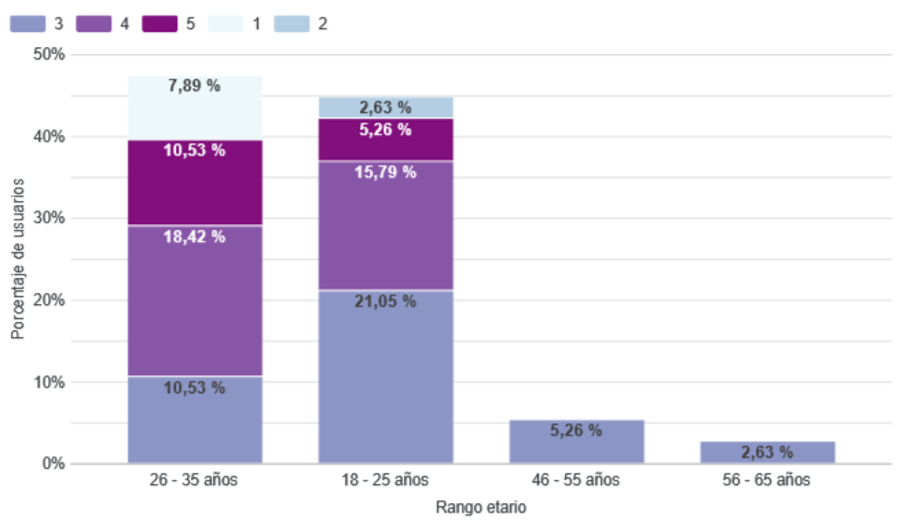
\includegraphics[width=0.90\textwidth]{figures/word/image4.png}
\caption{Nivel de dificultad para estimar el precio justo de alquiler según rango etario.}
\end{figure}

Al aislar el segmento de alquileres, se observa que el 65,79\% de los encuestados de todas las edades califican con 4 o 5 la dificultad para determinar si un precio es justo. Esta asimetría de información es el problema central que resuelve el modelo predictivo de Nidio.

\begin{figure}[htbp]
\centering
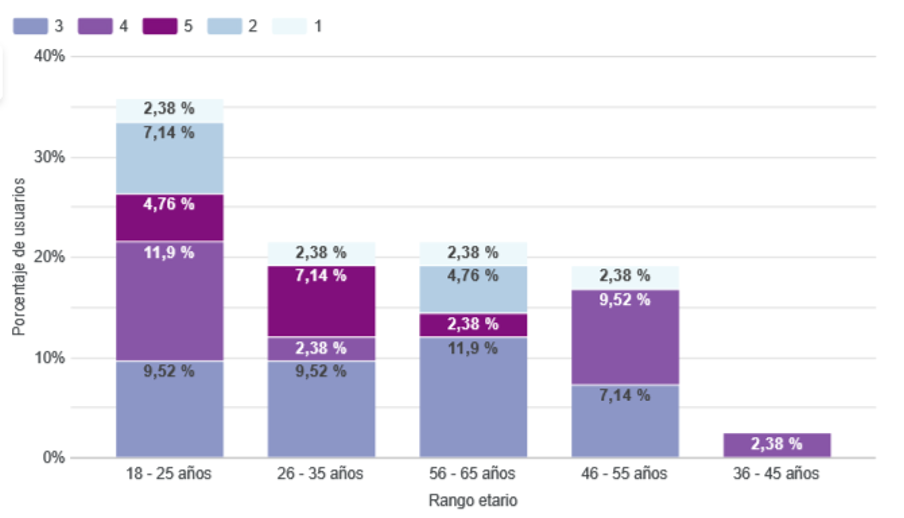
\includegraphics[width=0.90\textwidth]{figures/word/image7.png}
\caption{Nivel de dificultad para estimar el precio justo de compra según rango etario.}
\end{figure}

Al aislar el segmento de compra, se observa que el 40,46\% de los encuestados de todas las edades califican con 4 o 5 la dificultad para determinar si un precio para comprar una propiedad es justo. Nuevamente, se demuestra una asimetría de la información

\begin{figure}[htbp]
\centering
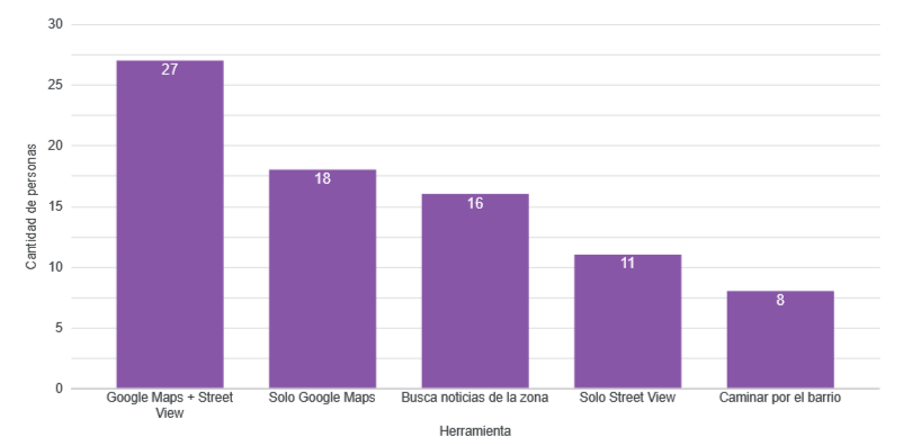
\includegraphics[width=0.90\textwidth]{figures/word/image9.png}
\caption{Acciones complementarias de investigación de zona realizadas por los usuarios.}
\end{figure}

El mercado actual obliga al usuario a utilizar herramientas de terceros. El 60,86\% de los usuarios debe recurrir a Google Maps o Street View de forma externa. Además, el 8,69\% decide caminar por el barrio para investigar la zona donde se encuentra la propiedad. La integración de la API de OpenStreetMap en Nidio centraliza esta experiencia, resolviendo una fricción directa del usuario.

\begin{figure}[htbp]
\centering
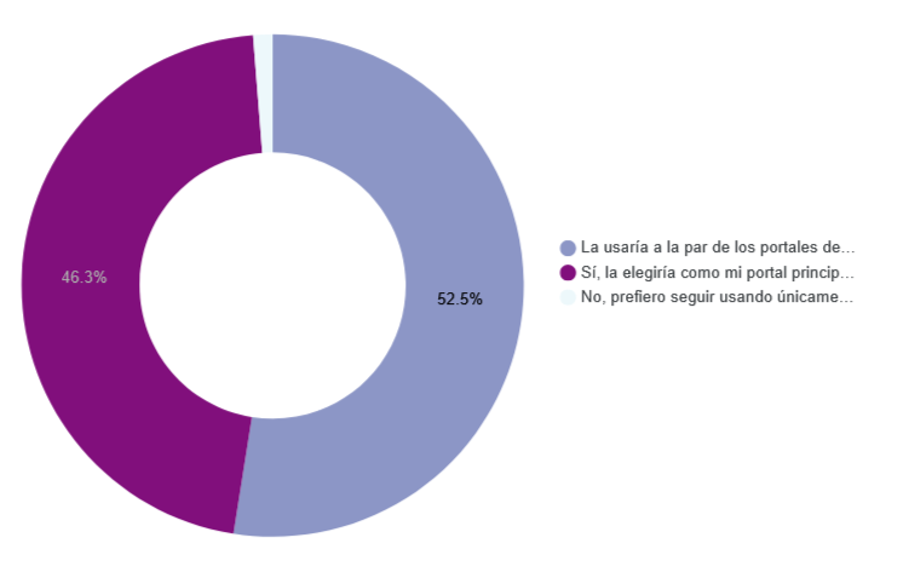
\includegraphics[width=0.90\textwidth]{figures/word/image17.png}
\caption{Comparativa de intención de adopción de Nidio frente a competidores.}
\end{figure}

A pesar del monopolio de plataformas como Zonaprop o Argenprop, una abrumadora cantidad de personas (el 46,3\%) indicó que cambiaría sus hábitos y elegiría a Nidio como portal principal si éste ofreciera análisis de datos objetivos. Además, el 52,5\% usaría Nidio a la par de los portales tradicionales, lo cual indica que el 98,8\% utilizaría nuestra plataforma.

\begin{figure}[htbp]
\centering
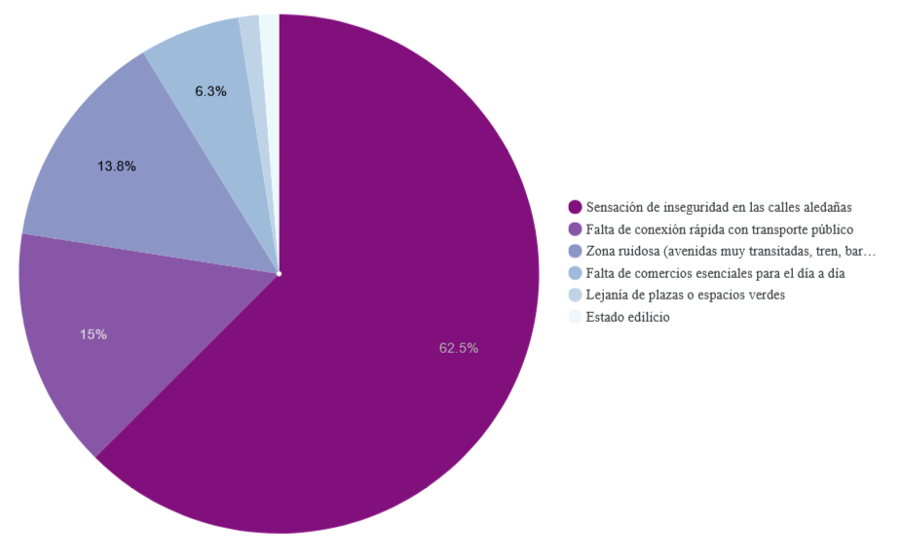
\includegraphics[width=0.90\textwidth]{figures/word/image3.png}
\caption{Mayor motivo de descarte de propiedad.}
\end{figure}

El factor ambiental no es secundario. Un 76,3\% de los encuestados consideró que el nivel de ruido y la seguridad son 'Indispensables' al momento de elegir una propiedad, validando la inclusión de estas variables en los mapas de calor de nuestra plataforma. Además, el 15\% cree indispensable la conexión al transporte público. Con nuestro Life Score, los usuarios podrán visualizar la cercanía a esos puntos de interés.

\begin{figure}[htbp]
\centering
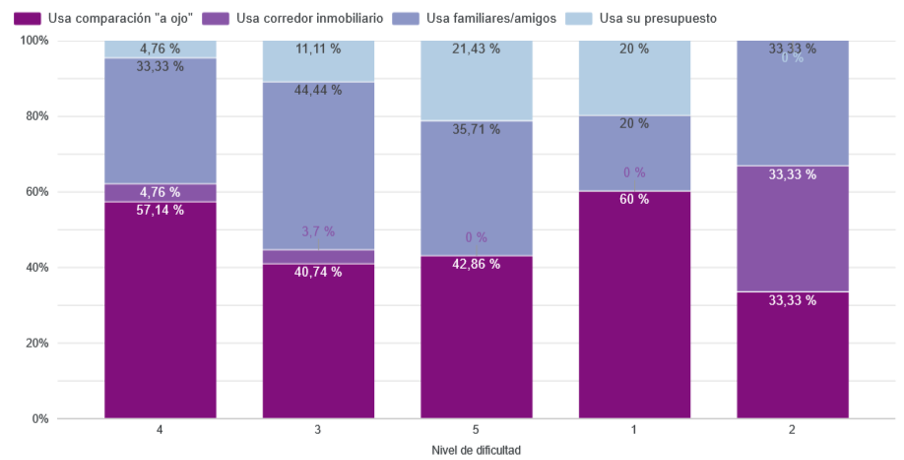
\includegraphics[width=0.90\textwidth]{figures/word/image13.png}
\caption{Distribución de respuestas sobre la influencia de Nidio en la decisión.}
\end{figure}

La figura 6 presenta la correlación entre la metodología de validación de precios de alquiler empleada por los usuarios y el nivel de dificultad (del 1 al 5 siendo 1 ``muy fácil'') percibido para detectar sobrevaluaciones al leer el precio de un alquiler. Se observa que los métodos basados en heurísticas informales (como la comparación visual o consultarle a familiares/amigos) presentan una mayor media de dificultad respecto a los métodos profesionales. Esta disparidad en la dificultad de validación del precio publicado valida la propuesta de Nidio como una solución que estandariza y automatiza el proceso de tasación, reduciendo la carga cognitiva del usuario y otorgando mayor certidumbre a la operación inmobiliaria. Figura 7. Nivel de desconfianza promedio por portal inmobiliario

\begin{figure}[htbp]
\centering
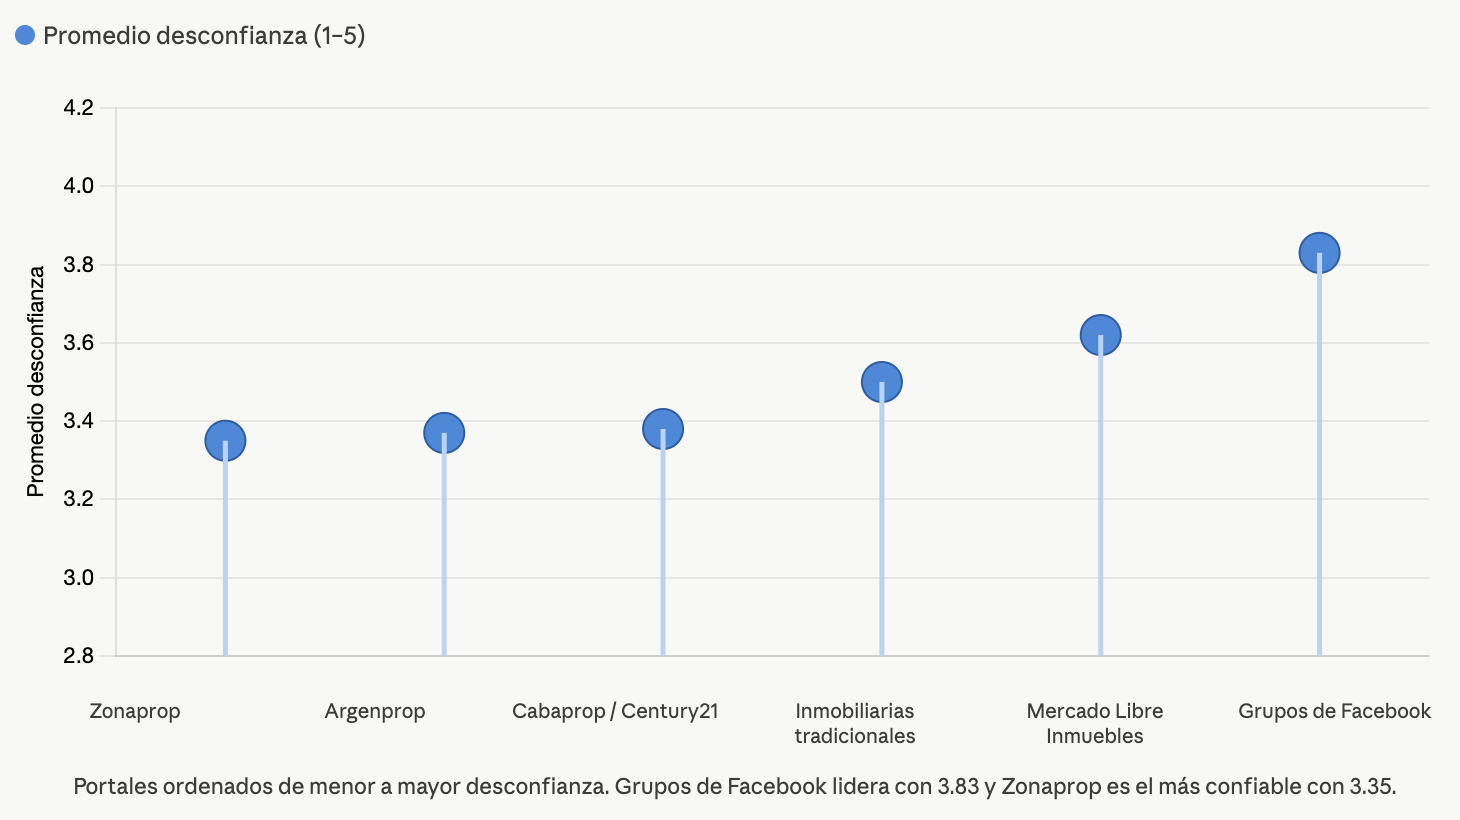
\includegraphics[width=0.90\textwidth]{figures/word/image18.png}
\caption{Promedio de importancia asignada a puntos de interés.}
\end{figure}

Los usuarios de portales inmobiliarios de CABA muestran niveles de desconfianza similares entre plataformas (entre 3.35 y 3.83 sobre 5). Grupos de Facebook presenta el mayor nivel de desconfianza (3.83), mientras que Zonaprop es el portal con valores más bajos (3.35). La escasa diferencia entre portales sugiere que la desconfianza en los precios publicados es una percepción generalizada, independiente de la plataforma utilizada.

\subsection{Entrevistas Cualitativas}

Con el objetivo de comprender las necesidades, frustraciones y comportamientos de los distintos actores del mercado inmobiliario de CABA, se realizaron entrevistas semiestructuradas a tres perfiles representativos: una agente inmobiliaria, una propietaria de varios inmuebles y una persona en proceso de compraventa. Las entrevistas fueron grabadas con consentimiento de los participantes y transcritas para su análisis. A continuación se presentan los hallazgos principales de cada entrevista.

\subsubsection{Entrevista 1 --- Agente Inmobiliaria}

La primera entrevistada es Sharon, agente inmobiliaria con 3 años de experiencia en el rubro, con base en Palermo, CABA. La entrevista permitió relevar el proceso de tasación y publicación de propiedades desde el lado profesional del mercado. Sharon describió que el proceso de tasación es empírico y basado en la experiencia acumulada: se toman como referencia propiedades similares en la misma zona considerando metros cuadrados, ambientes y amenities, y se negocia el precio con el propietario. Si el precio solicitado está fuera de mercado y el propietario no cede, la propiedad directamente no se publica. Respecto a las consultas de los clientes, Sharon señaló que la información más solicitada es el precio real al que el propietario está dispuesto a ceder, si la propiedad está fuera de valor según su criterio y cuánto tiempo lleva publicada. También destacó que el entorno juega un papel determinante en la decisión de compra o alquiler: los clientes consultan sistemáticamente sobre acceso a transporte público, cercanía a supermercados, hospitales y escuelas, y presencia de plazas o shoppings en los alrededores. En cuanto a las herramientas digitales, Sharon las considera esenciales para el trabajo diario, principalmente para consultar el mercado actualizado, publicar propiedades y comparar tasaciones. Identificó como una mejora deseable que una aplicación pueda determinar el valor real de una propiedad mediante inteligencia artificial, reduciendo la subjetividad del proceso de tasación. También mencionó que le gustaría poder mostrarle al cliente el entorno de la propiedad directamente desde una herramienta digital, algo que hoy no hace pero que considera que sumaría mucho valor. Los hallazgos de esta entrevista validan dos componentes centrales de Nidio: el modelo de valuación basado en ML como respuesta a la subjetividad del proceso de tasación tradicional, y el Life Score como herramienta para comunicar objetivamente el entorno urbano de una propiedad sin necesidad de recorrerlo físicamente.

\subsubsection{Entrevista 2 --- Propietaria de Varios Inmuebles}

La segunda entrevistada es Madelaine, propietaria e inversora con más de 15 años de experiencia gestionando un portfolio de inmuebles en CABA. La entrevista permitió relevar las fricciones en la administración de alquileres, los procesos de tasación y el análisis de zonas para inversión desde la óptica del dueño directo. Madelaine describió que actualmente prefiere gestionar sus propiedades de manera directa. Su experiencia delegando en inmobiliarias tradicionales es mixta: si bien reconoce que son ágiles para conseguir inquilinos, señaló que suelen desentenderse de la administración y los problemas legales posteriores. Para fijar los precios de alquiler o venta, se basa en la observación manual de portales y en tasaciones históricas, aunque destacó la dificultad de mantener los precios actualizados a lo largo del tiempo, sufriendo desfases en los contratos por no contar con información de mercado accesible y en tiempo real. Respecto al uso de plataformas inmobiliarias tradicionales, señaló que prefiere evitarlas debido a la falta de herramientas de validación de perfiles. Su mayor temor radica en la inseguridad jurídica y el cuidado del inmueble, por lo que prioriza el ``boca a boca'' y las recomendaciones de inquilinos de confianza, evidenciando una falta de confianza en los portales actuales que operan como simples carteleras. A la hora de evaluar una nueva propiedad como inversión, Madelaine remarcó que el entorno es fundamental. Analiza la popularidad del barrio, la seguridad y la conectividad mediante transporte público, enfocándose en las necesidades de su público objetivo (estudiantes y trabajadores). Sin embargo, indicó que la investigación de estos factores es tediosa y poco fiable, ya que actualmente ``no existe una página donde se puedan ver todos los detalles reales del barrio'', obligándola a depender de búsquedas manuales en internet o referencias de conocidos. En cuanto a su herramienta digital ideal, destacó la necesidad de una plataforma centralizada. Específicamente, mencionó que le solucionaría un gran problema contar con un sistema que le brinde un rango de precios predefinido por zona, permitiéndole saber objetivamente cuánto vale su propiedad sin ``regalarla ni aprovecharse''. También sugirió la necesidad de integrar validaciones de usuarios con historial previo de alquileres (estilo Airbnb) y facilidades legales, como pre-contratos y firmas digitales. Los hallazgos de esta entrevista validan empíricamente los dos pilares de Nidio: el modelo predictivo de valuación (AVM) responde a la necesidad explícita de la inversora de obtener rangos de precios objetivos y actualizados para evitar el desfase de valores; y el Life Score, junto con los mapas de calor, resuelven de forma directa su frustración ante la falta de información centralizada sobre el entorno urbano y la seguridad al momento de invertir. 2.3.2.3. Entrevista 3 --- Persona en Proceso de Compraventa

% TODO: contenido pendiente en el documento Word original.

\subsection{Arquetipos de Usuario}

Con el objetivo de caracterizar a los potenciales usuarios de Nidio, se desarrollaron tres User Persona que representan los perfiles principales de compradores e inquilinos en el mercado inmobiliario de CABA. Cada perfil fue construido a partir del análisis de la problemática identificada en el Capítulo 1 y de los hallazgos obtenidos en las entrevistas realizadas.

\subsubsection{El Estudiante Universitario --- Inquilino Primerizo}

Tomás representa al usuario que enfrenta por primera vez el mercado de alquiler en una ciudad que no conoce. Su principal necesidad es acceder a información objetiva sobre conectividad y seguridad del entorno, variables que los portales tradicionales no ofrecen. Es un nativo digital con alta receptividad a herramientas analíticas y toma decisiones desde dispositivos móviles.

\begin{figure}[htbp]
\centering
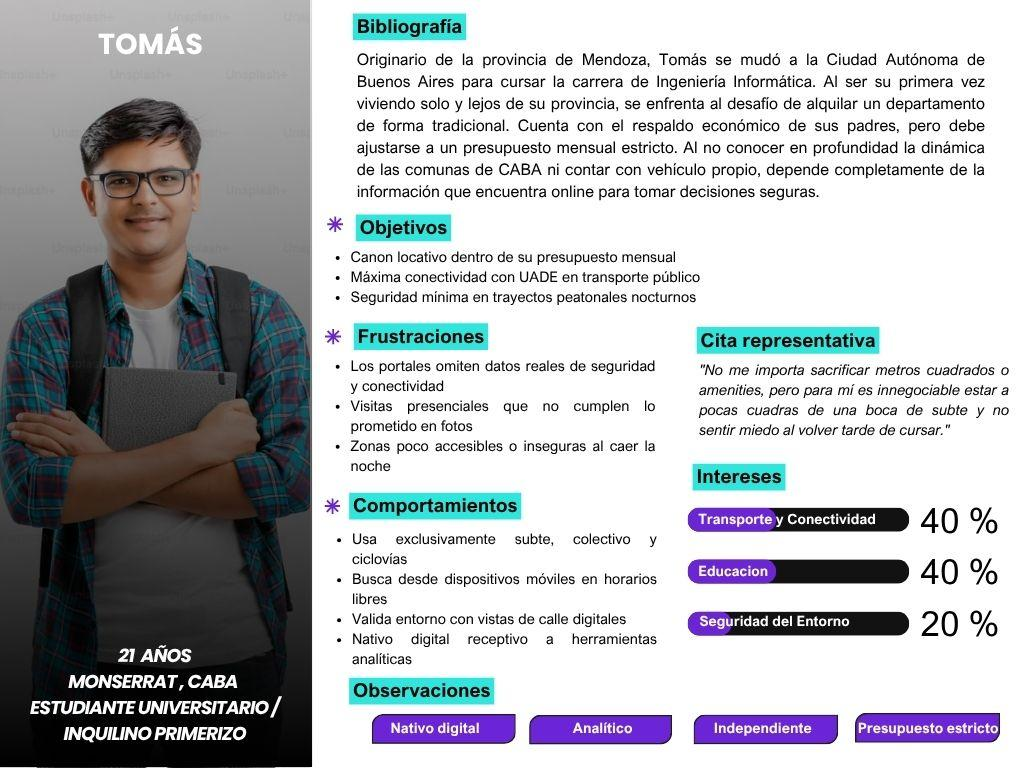
\includegraphics[width=0.90\textwidth]{figures/word/image15.jpg}
\caption{User Persona: estudiante universitario e inquilino primerizo.}
\end{figure}

\subsubsection{La Pareja Profesional --- Inquilinos con Experiencia}

Camila y Federico representan al usuario que ya conoce la dinámica del mercado pero necesita validar con datos objetivos si los precios están justificados respecto al entorno. Trabajan bajo modalidad híbrida y priorizan el lifestyle por sobre la conectividad laboral. Su frustración central es la falta de transparencia sobre el valor real de las zonas.

\begin{figure}[htbp]
\centering
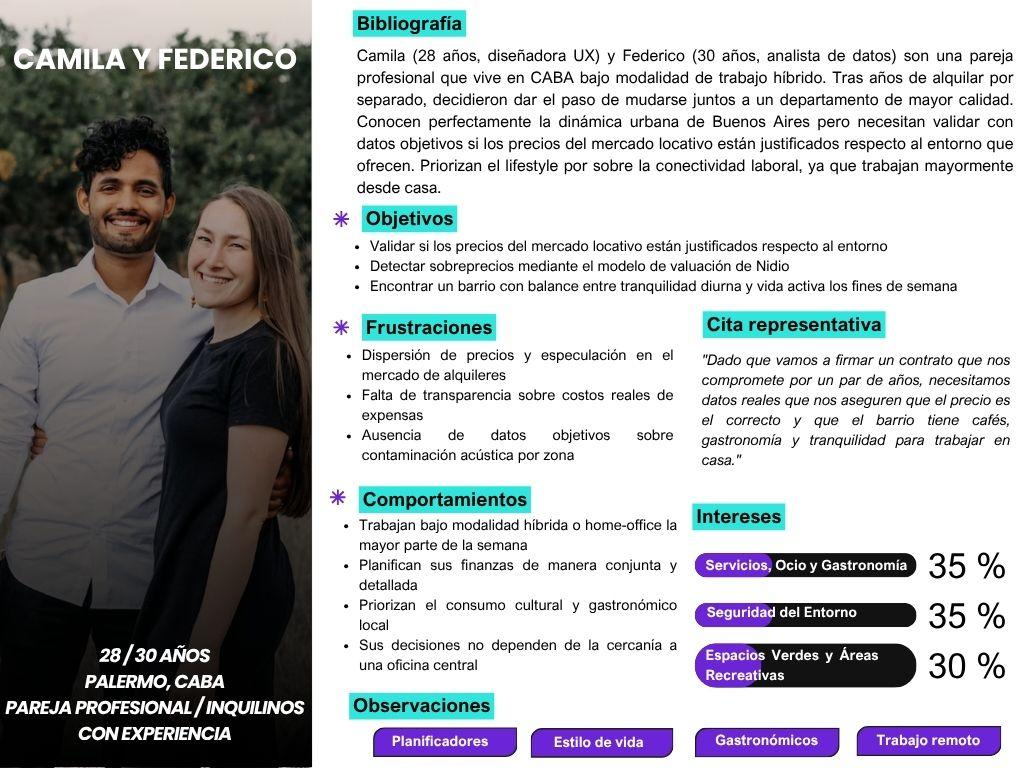
\includegraphics[width=0.90\textwidth]{figures/word/image16.jpg}
\caption{User Persona: pareja profesional e inquilinos con experiencia.}
\end{figure}

\subsubsection{La Familia Joven --- Compradores de Primera Vivienda}

Laura y Martín representan al usuario que enfrenta la decisión de mayor impacto económico de su vida. Necesitan auditar técnicamente el precio por metro cuadrado y evaluar con datos empíricos la calidad del entorno para la crianza. Son los únicos del conjunto que ponen a prueba el modelo de valuación de venta en dólares.

\begin{figure}[htbp]
\centering
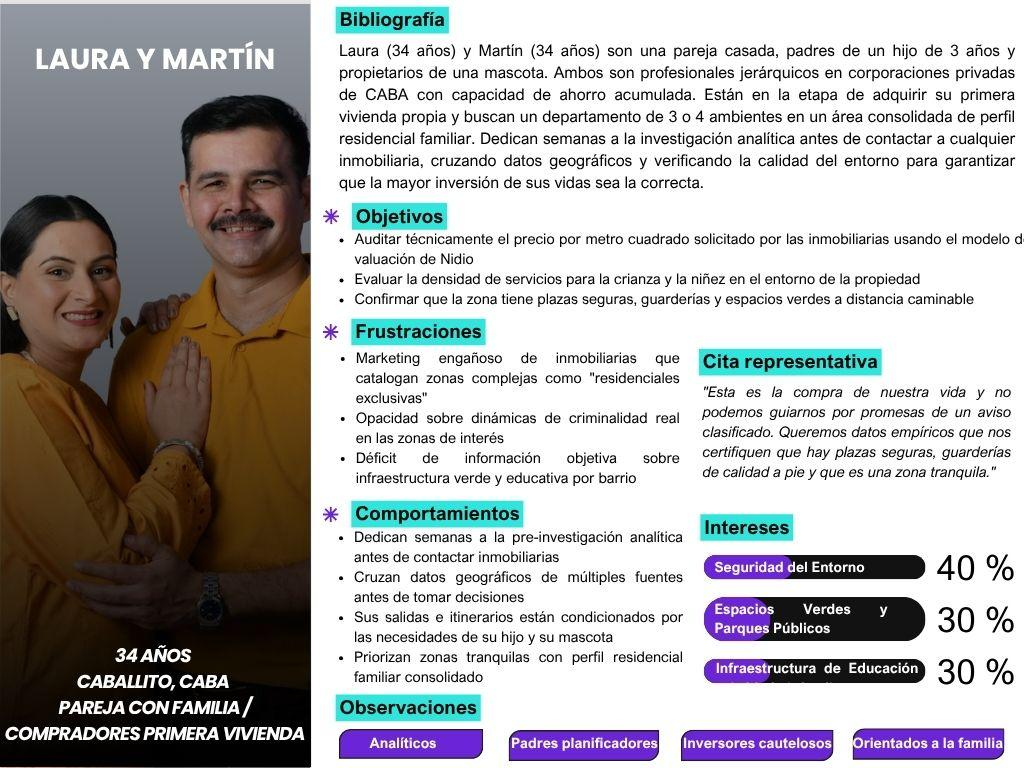
\includegraphics[width=0.90\textwidth]{figures/word/image14.jpg}
\caption{User Persona: familia joven y compradores de primera vivienda.}
\end{figure}

\section{Aspectos Legales y Éticos}

\subsection{Ley de Protección de Datos Personales (Ley N° 25.326)}

El desarrollo de la plataforma Nidio conlleva el procesamiento de grandes volúmenes de información inmobiliaria. Para garantizar un enfoque ético y minimizar los riesgos legales, la arquitectura de datos del proyecto se diseñó en estricto cumplimiento con la Ley Nacional N° 25.326 de Protección de los Datos Personales \parencite{ArgentinaLey25326}.

\subsection{Definición de Datos Personales y Alcance}

De acuerdo con el Artículo 2° de la citada ley, se entiende por datos personales a la ``información de cualquier tipo referida a personas físicas o de existencia ideal determinadas o determinables''. En el contexto de los portales inmobiliarios tradicionales, esto abarca elementos críticos de las publicaciones, tales como:

\begin{itemize}
\item Nombre y apellido del propietario o agente inmobiliario.
\item Números de teléfono y direcciones de correo electrónico de contacto.
\item Dirección exacta (calle, altura, piso y departamento) que permite la identificación única del inmueble y, por extensión, de sus ocupantes o dueños.
\end{itemize}

El almacenamiento de estos datos en los servidores de la plataforma sometería al proyecto a obligaciones jurídicas estrictas respecto a la custodia y privacidad de la información.

\subsection{2.4.3. El Principio del Consentimiento}

El pilar fundamental que restringe la extracción automatizada de datos reales de la competencia es el Artículo 5°, el cual establece explícitamente que ``el tratamiento de datos personales es ilícito cuando el titular no hubiere prestado su consentimiento libre, expreso e informado''. Si bien los datos de contacto y ubicación pueden estar publicados y ser visibles en plataformas de terceros, el Artículo 4°, inciso 3, determina que ``los datos objeto de tratamiento no pueden ser utilizados para finalidades distintas o incompatibles con aquellas que motivaron su obtención''. Por lo tanto, recopilar información de individuos que otorgaron su consentimiento a un portal específico, para luego almacenarla y procesarla en los servidores de Nidio sin un acuerdo expreso y por escrito, constituiría una infracción a la normativa vigente.

\subsection{2.4.4. Decisión Arquitectónica y Privacidad desde el Diseño}

Como consecuencia de estas restricciones legales, el proyecto descarta de plano el uso de mecanismos de recolección de datos que vulneren la privacidad de los usuarios. En su lugar, a nivel arquitectónico, se optó por el desarrollo de una base de datos sintética de inmuebles para la capa de servicios (Backend). Esta decisión tecnológica permite simular las publicaciones y validar de manera integral todos los flujos de uso de la aplicación web, evitando por completo el almacenamiento de datos reales amparados por la Ley N° 25.326 y garantizando que el prototipo funcional (MVP) sea un producto ético y legalmente viable desde su concepción. Si bien la extracción automatizada de datos (web scraping) es una técnica estandarizada en la ingeniería de datos para la ingesta de grandes volúmenes de información, su aplicación sobre los portales inmobiliarios comerciales del mercado local presenta un obstáculo legal y ético insalvable. El acceso y la navegación en plataformas líderes como Zonaprop y Argenprop están regidos por Términos y Condiciones de Uso que funcionan como contratos de adhesión vinculantes para cualquier usuario o sistema automatizado que interactúe con ellas.

\subsection{Violación de Propiedad Intelectual y Extracción de Bases de Datos}

El análisis de los términos legales de las principales plataformas competidoras revela prohibiciones explícitas orientadas a proteger sus bases de datos como activos de propiedad intelectual. En el caso de Argenprop (2026), la plataforma detalla en su apartado de ``Marcas registradas, Derechos de autor y restricciones'' una prohibición directa a la técnica de scraping, estableciendo textualmente que: ``El usuario acepta no utilizar el sitio web ni los materiales incluidos o extraídos del sitio web de manera ilegal, lo que incluye, sin carácter restrictivo, extraer (scraping) contenido del sitio o la base de datos para obtener listas de inventario u otra información privada.'' Asimismo, prohíbe taxativamente ``usar cualquier mecanismo, software o rutina para impedir o intentar impedir el adecuado funcionamiento'' de su sitio, así como ``intentar descifrar, descompilar u obtener el código fuente'' de su arquitectura web. Por su parte, los términos de servicio de Zonaprop (2026) refuerzan esta protección mediante la cláusula de ``Cesión o Uso Comercial No Autorizado'', donde en su Artículo 7.1 el usuario ``acepta no realizar ningún uso comercial no autorizado del Sitio Web''. El despliegue de crawlers o arañas web para replicar sus listados de propiedades con el fin de alimentar el modelo de Nidio constituiría un aprovechamiento comercial no autorizado de su infraestructura técnica y comercial.

\subsection{Conclusión Arquitectónica}

Ignorar estas restricciones e implementar módulos de scraping en la capa de ingesta de datos (Backend) expondría al proyecto Nidio a conflictos por infracción de derechos de autor, violación de contratos de uso corporativos y prácticas de competencia desleal. Por consiguiente, para salvaguardar la viabilidad legal y el rigor ético del Proyecto Final de Ingeniería, se descarta por completo la extracción automatizada de portales de terceros, sentando la base para la adopción de fuentes de datos abiertas y la generación de bases de datos sintéticas para entornos de prueba.

\subsection{Justificación del uso de Base de Datos Sintética}

Ante la imposibilidad legal y contractual de extraer bases de datos reales mediante técnicas de web scraping (como se detalló en las secciones anteriores), el proyecto requiere una alternativa técnica robusta para poblar el catálogo de la plataforma web y ejecutar pruebas integrales del sistema (Quality Assurance y End-to-End). Para ello, se optó por la generación de una base de datos sintética. En la ingeniería de software moderna, la generación de datos sintéticos es un estándar de la industria para evaluar la fiabilidad y el comportamiento de sistemas intensivos en datos. La literatura especializada establece que, para que las pruebas basadas en el uso del sistema sean efectivas, los datos de prueba generados artificialmente deben cumplir con dos restricciones fundamentales: representatividad estadística y validez lógica \parencite{SoltanaEtAl2017}. En el contexto del desarrollo de la plataforma Nidio, la generación del dataset mediante scripts (utilizando librerías especializadas como Faker en Python) se alinea estrictamente con estos principios:

\begin{itemize}
\item \textbf{Por empezar, la representatividad estadística.} Los datos ficticios generados (como precios, superficies y cantidad de ambientes) no son puramente aleatorios, sino que se parametrizan para seguir distribuciones estadísticas que reflejan el estado actual del mercado inmobiliario real. Esto asegura que la experiencia del usuario al navegar, filtrar y utilizar el modelo de valuación en el prototipo funcional (MVP) sea equivalente a interactuar con un entorno de producción.
\item \textbf{Además, la validez lógica (logical constraints).} El algoritmo de generación de datos impone reglas de negocio estrictas para evitar anomalías lógicas. Por ejemplo, las coordenadas geográficas (latitud y longitud) están limitadas a los polígonos correspondientes a la Ciudad Autónoma de Buenos Aires (CABA); y la relación entre tipo de propiedad, metros cuadrados y precio se mantiene dentro de rangos coherentes.
\end{itemize}

En conclusión, la adopción de una base de datos sintética no solo garantiza el cumplimiento absoluto de la Ley de Protección de Datos Personales y los derechos de propiedad intelectual de terceros, sino que proporciona un entorno de pruebas escalable y controlado que valida con rigor la arquitectura técnica del proyecto.

\subsection{Licencias de Fuentes Abiertas (OpenStreetMap, IDECBA, Kaggle)}

El proyecto se apoya exclusivamente en datos de libre acceso para garantizar la legalidad del enfoque y la reproducibilidad del trabajo.

\begin{center}
\small
\begin{longtable}{|p{0.22\textwidth}|p{0.20\textwidth}|p{0.18\textwidth}|p{0.28\textwidth}|}
\caption{Licencias de fuentes abiertas}\label{tab:licencias}\\
\hline
Fuente & Tipo de dato & Licencia & Permisos y condiciones \\
\hline
\endfirsthead
\hline
Fuente & Tipo de dato & Licencia & Permisos y condiciones \\
\hline
\endhead
Kaggle (Datasets inmobiliarios) & Individual & Apache 2.0 / MIT & Uso comercial, modificación y distribución permitidos con atribución. \\
\hline
Properati (Datasets) & Individual & CC BY-SA 3.0 & Uso comercial permitido, requiere atribución y compartir bajo la misma licencia. \\
\hline
IDECBA y BA Data (Datasets) & Agregado & CC BY 2.5 AR & Uso comercial permitido, requiere atribución al organismo emisor. \\
\hline
OpenStreetMap & Geoespacial & ODbL & Uso libre, requiere atribución y compartir bajo la misma licencia. \\
\hline
\end{longtable}
\end{center}
